\documentclass{report}
\usepackage[spanish]{babel}
\usepackage[utf8]{inputenc}
\usepackage{graphicx, longtable, float, titlesec, hyperref, enumitem, dingbat, soul, multicol, listings}
\usepackage[dvipsnames]{xcolor}
\usepackage[margin=2cm]{geometry}

% Cambia el color de los links
\hypersetup{
    hidelinks = true
}

% Python Code
\lstdefinestyle{Python}{
  commentstyle=\color{brown},
  keywordstyle=\color{violet},
  numberstyle=\tiny\color{gray},
  stringstyle=\color{purple},
  basicstyle=\ttfamily\footnotesize,
  breakatwhitespace=false,         
  breaklines=true,                 
  captionpos=b,                    
  keepspaces=true,                 
  numbers=left,                    
  numbersep=5pt,                  
  showspaces=false,                
  showstringspaces=false,
  showtabs=false,                  
  tabsize=2,
  literate={ñ}{{\~n}}1 {á}{{\'a}}1 {é}{{\'e}}1 {í}{{\'i}}1 {ó}{{\'o}}1 {ú}{{\'u}}1
}
\lstset{style=Python}

% Elimina la palabra "Capítulo" de los títulos de los capítulos
\titleformat{\chapter}[display]
  {\normalfont\bfseries}{}{0pt}{\Huge\thechapter.\space}

\titleformat{name=\chapter,numberless}[display]
  {\normalfont\bfseries}{}{0pt}{\Huge}

\titlespacing*{\chapter}{0pt}{-50pt}{20pt}

% Personalización del índice de listados
\renewcommand{\lstlistingname}{Código}  % Cambiar el nombre de "Listing" a "Código"
\renewcommand{\lstlistlistingname}{Índice de Códigos}

% Añade numeración a los subsubsection*s y los añade al índice
\setcounter{secnumdepth}{4}
\setcounter{tocdepth}{4}

\begin{document}
    \begin{titlepage}
        \centering
        
\includegraphics[width=0.6\textwidth]{./.img/logo.jpg}\\
        \vspace{1cm}
        \LARGE Técnicas de Inteligencia Artificial\\
        \vspace{0.5cm}
        \Large Ingeniería Informática de Gestión y Sistemas de Información\\
        \vspace{3cm}
        \Huge Practica 2\\
        \huge Búsqueda Multi-Agente\\
        \vspace{2.5cm}
        \Large Autor(es):\\
        \vspace{0.2cm}
        \large Xabier Gabiña\\
        \large Diego Montoya\\
        \vfill
        \today
    \end{titlepage}
    \tableofcontents
    \listoffigures
    \lstlistoflistings
    \chapter{Introducción}
      \paragraph*{}{
        En esta práctica se implementarán varios algoritmos de búsqueda multi-agente para el juego de Pacman. 
        Los algoritmos a implementar son los siguientes:
        \begin{itemize}
          \item Agente Reflex: Un agente que selecciona acciones a corto plazo basándose en la percepción actual del entorno.
          \item Minimax: Un algoritmo de búsqueda en árboles que se utiliza en juegos de dos o más jugadores y deterministas.
          \item Podado Alpha-Beta: Una mejora del algoritmo Minimax que reduce el número de nodos evaluados en el árbol de búsqueda.
          \item Expectimax: Una variante del algoritmo Minimax que se utiliza cuando los oponentes no toman siempre la mejor decisión posible.
        \end{itemize}
        Además, se mejorará la función de evaluación del agente reflex para que tome en cuenta más factores del estado del juego.
      }
    \chapter{Ejercicios}
      \section{Agente Reflex}
        \subsection*{Descripción}
          \paragraph*{}{
            Un agente reflex es un agente que selecciona acciones a corto plazo basándose en la percepción actual del entorno. 
            En este caso, el agente reflex se basa en una función de evaluación para seleccionar la mejor acción en cada estado. 
            La función de evaluación asigna un valor numérico a cada estado, y el agente selecciona la acción que maximiza este valor.
            Para asignar un valor a cada estado, la función de evaluación considera varios factores, como la distancia a la comida, la proximidad a los fantasmas y la cantidad de comida restante.
          }
        \subsection*{Primera implementación}
          \begin{lstlisting}[language=Python, caption=Implementación inicial del agente reflex]
          \end{lstlisting}
        \subsection*{Implementación final}
          \begin{lstlisting}[language=Python, caption=Implementación final del agente reflex]
class ReflexAgent(Agent):
  """
  Un agente reflexivo que elige acciones basándose en una función de evaluación.
  """

  def getAction(self, gameState):
      """
      Devuelve la mejor acción para Pacman basada en la función de evaluación.
      """
      # Obtiene las acciones legales para Pacman
      legalMoves = gameState.getLegalActions()

      # Calcula los puntajes para cada acción utilizando la función de evaluación
      scores = [self.evaluationFunction(gameState, action) for action in legalMoves]
      bestScore = max(scores)  # Encuentra el puntaje más alto
      bestIndices = [index for index in range(len(scores)) if scores[index] == bestScore]
      chosenIndex = random.choice(bestIndices)  # Elige aleatoriamente entre las mejores acciones

      return legalMoves[chosenIndex]

  def evaluationFunction(self, currentGameState, action):
      """
      Calcula el valor del estado sucesor después de que Pacman toma la acción `action`.
      Devuelve un valor numérico mayor para estados más favorables.
      """
      # Generar el estado sucesor
      successorGameState = currentGameState.generatePacmanSuccessor(action)
      # Obtiene la posición de Pacman después de moverse
      newPos = successorGameState.getPacmanPosition()
      # Obtiene la matriz de comida en el estado sucesor
      newFood = successorGameState.getFood()
      # Obtiene la lista de estados de los fantasmas
      newGhostStates = successorGameState.getGhostStates()
      # Obtiene los tiempos restantes de los fantasmas asustados
      newScaredTimes = [ghostState.scaredTimer for ghostState in newGhostStates]

      # Inicializar el puntaje con el puntaje base del sucesor
      score = successorGameState.getScore()

      # 1. Distancia a la comida más cercana
      foodList = newFood.asList()  # Convertir la matriz de comida a una lista de posiciones
      if foodList:  # Si hay comida disponible
          # Calcular la distancia mínima a la comida más cercana
          minFoodDistance = min([manhattanDistance(newPos, food) for food in foodList])
          # Invertir la distancia para que un menor valor de distancia dé un mayor puntaje
          score += 10.0 / minFoodDistance

      # 2. Distancia a los fantasmas no asustados
      for ghost in newGhostStates:
          ghostPos = ghost.getPosition()
          ghostDistance = manhattanDistance(newPos, ghostPos)
          if ghostDistance < 2 and ghost.scaredTimer == 0:  # Fantasma no asustado y muy cerca
              score -= 1000  # Penalización fuerte por estar demasiado cerca de un fantasma peligroso

      # 3. Incentivo por acercarse a fantasmas asustados
      for i, ghost in enumerate(newGhostStates):
          if newScaredTimes[i] > 0:  # Si el fantasma está asustado
              ghostDistance = manhattanDistance(newPos, ghost.getPosition())
              score += 200.0 / (ghostDistance + 1)  # Premiar estar cerca de un fantasma asustado

      # 4. Penalización por comida restante
      score -= len(foodList) * 10  # Penalizar por cada comida restante en el estado sucesor

      return score
          \end{lstlisting}
        \subsection*{Comentarios}
          \paragraph*{}{

          }
      \clearpage\section{Minimax}
        \subsection*{Descripción}
          \paragraph*{}{
            Minimax es un algoritmo de búsqueda en árboles que se utiliza en juegos de dos o más jugadores y deterministas.
            El algoritmo Minimax se basa en la idea de que los jugadores intentan maximizar su puntaje, mientras que sus oponentes intentan minimizarlo, es decir, juegos de suma cero.
            Este algoritmo es especialmente útil cuando el oponente toma siempre la mejor decisión posible.

            El algoritmo Minimax funciona de la siguiente manera:
            \begin{enumerate}
                \item Se construye un árbol de busqueda con todos los posibles movimientos.
                \item Cada nodo del árbol representa un estado del juego y cada rama representa una acción.
                \item El arbol alterna entre los jugadores, uno intenta maximizar el puntaje y los otros minimizarlo.
                \item Se evaluan los nodos terminales del árbol y se asigna un valor usando una función de evaluación.
                \item Dependiendo del jugador, se selecciona el nodo hijo con el valor máximo o mínimo.
            \end{enumerate}
            \begin{figure}[H]
                \centering
                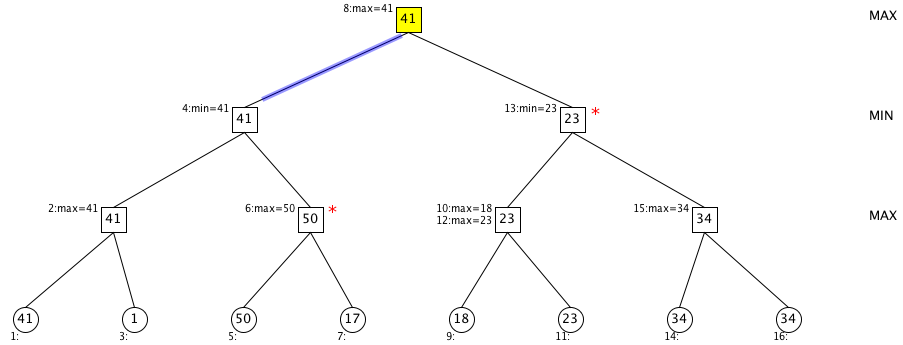
\includegraphics[width=0.9\textwidth]{./.img/minimax.png}
                \caption{Ejemplo de árbol de búsqueda Minimax}
            \end{figure}
            
            Respecto al coste tanto en tiempo como en espacio, el algoritmo Minimax es, en esencia un DFS por lo que su coste en tiempo es $O(b^m)$ y en espacio $O(bm)$. 
            Estos malos costes se deben a que el algoritmo explora todo el árbol de búsqueda, lo que lo hace inviable en juegos con un gran factor de ramificación y profundidad.
          }
        \subsection*{Primera implementación}
          \begin{lstlisting}[language=Python, caption=Implementación inicial del agente Minimax]
class MinimaxAgent(MultiAgentSearchAgent):
  """
  Agente que implementa el algoritmo Minimax.
  """

  def getAction(self, gameState):
      """
      Devuelve la mejor acción para Pacman desde el estado actual `gameState` usando Minimax.
      """
      # Llama a la función minimax empezando con el agente 0 (Pacman) y profundidad 0
      best_action, _ = self.minimax(gameState, agentIndex=0, depth=0)
      return best_action

  def minimax(self, gameState, agentIndex, depth):
      """
      Función minimax que devuelve la mejor acción y su valor para el agente actual.
      """
      # Si el estado es terminal (gana o pierde) o alcanzamos la profundidad máxima, evaluamos el estado
      if gameState.isWin() or gameState.isLose() or depth == self.depth:
          return None, self.evaluationFunction(gameState)

      if agentIndex == 0: # Pacman - Maximizador
          return self.max_value(gameState, agentIndex, depth)
      else:               # Fantasmas - Minimizadores
          return self.min_value(gameState, agentIndex, depth)

  def max_value(self, gameState, agentIndex, depth):
      """
      Calcula el valor máximo para el agente Pacman (maximizador).
      """
      # Inicializar el mejor valor y la mejor acción
      best_value = float('-inf')
      best_action = None

      # Recorre todas las acciones legales para Pacman
      for action in gameState.getLegalActions(agentIndex):
          # Generar el estado sucesor
          successorState = gameState.generateSuccessor(agentIndex, action)
          # Calcular el valor del sucesor usando minimax con el siguiente agente
          _, successor_value = self.minimax(successorState, 1, depth)
          # Actualiza el valor máximo si se encuentra un mejor valor
          if successor_value > best_value:
              best_value = successor_value
              best_action = action

      return best_action, best_value

  def min_value(self, gameState, agentIndex, depth):
      """
      Calcula el valor mínimo para los fantasmas (minimizador).
      """
      # Inicializar el peor valor y la mejor acción
      worst_value = float('inf')
      best_action = None

      # Recorre todas las acciones legales para el fantasma actual
      for action in gameState.getLegalActions(agentIndex):
          # Generar el estado sucesor
          successorState = gameState.generateSuccessor(agentIndex, action)
          # Calcula el valor del sucesor con Pacman y siguiente nivel de profundidad
          _, successor_value = self.minimax(successorState, 0, depth + 1)

          # Actualiza el valor mínimo si se encuentra un peor valor
          if successor_value < worst_value:
              worst_value = successor_value
              best_action = action

      return best_action, worst_value

          \end{lstlisting}
        \subsection*{Implementación final}
          \begin{lstlisting}[language=Python, caption=Implementación final del agente Minimax]
class MinimaxAgent(MultiAgentSearchAgent):
  """
  Agente que implementa el algoritmo Minimax.
  """

  def getAction(self, gameState):
      """
      Devuelve la mejor acción para Pacman desde el estado actual `gameState` usando Minimax.
      """
      # Llama a la función minimax empezando con el agente 0 (Pacman) y profundidad 0
      best_action, _ = self.minimax(gameState, agentIndex=0, depth=0)
      return best_action

  def minimax(self, gameState, agentIndex, depth):
      """
      Función minimax que devuelve la mejor acción y su valor para el agente actual.
      """
      # Si el estado es terminal (gana o pierde) o alcanzamos la profundidad máxima, evaluamos el estado
      if gameState.isWin() or gameState.isLose() or depth == self.depth:
          return None, self.evaluationFunction(gameState)

      if agentIndex == 0: # Pacman - Maximizador
          return self.max_value(gameState, agentIndex, depth)
      else:               # Fantasmas - Minimizadores
          return self.min_value(gameState, agentIndex, depth)

  def max_value(self, gameState, agentIndex, depth):
      """
      Calcula el valor máximo para el agente Pacman (maximizador).
      """
      # Inicializar el mejor valor y la mejor acción
      best_value = float('-inf')
      best_action = None

      # Recorre todas las acciones legales para Pacman
      for action in gameState.getLegalActions(agentIndex):
          # Generar el estado sucesor
          successorState = gameState.generateSuccessor(agentIndex, action)
          # Calcular el valor del sucesor usando minimax con el siguiente agente
          _, successor_value = self.minimax(successorState, agentIndex + 1, depth)
          # Actualiza el valor máximo si se encuentra un mejor valor
          if successor_value > best_value:
              best_value = successor_value
              best_action = action

      return best_action, best_value

  def min_value(self, gameState, agentIndex, depth):
      """
      Calcula el valor mínimo para los fantasmas (minimizador).
      """
      # Inicializar el peor valor y la mejor acción
      worst_value = float('inf')
      best_action = None

      # Recorre todas las acciones legales para el fantasma actual
      for action in gameState.getLegalActions(agentIndex):
          # Generar el estado sucesor
          successorState = gameState.generateSuccessor(agentIndex, action)
          
          # Si es el último fantasma, pasamos a Pacman incrementando la profundidad
          if agentIndex == gameState.getNumAgents() - 1:
              # Calcula el valor del sucesor con Pacman y siguiente nivel de profundidad
              _, successor_value = self.minimax(successorState, 0, depth + 1)
          else:
              # Calcula el valor del sucesor con el siguiente fantasma
              _, successor_value = self.minimax(successorState, agentIndex + 1, depth)

          # Actualiza el valor mínimo si se encuentra un peor valor
          if successor_value < worst_value:
              worst_value = successor_value
              best_action = action

      return best_action, worst_value
        
          \end{lstlisting}
        \subsection*{Comentarios}
          \paragraph*{}{
            En la primera implementación no he tenido en cuenta el número de agentes, por lo que el algoritmo solo funcionaba con dos agentes. En la implementación final, he tenido en cuenta el número de agentes y he modificado la función \texttt{min\_value} para que si el agente actual es el último fantasma, pase a Pacman y aumente la profundidad.
          }
      \clearpage\section{Podado Alpha-Beta}
        \subsection*{Descripción}
          \paragraph*{}
          {
            El algoritmo Alpha-Beta es una mejora del algoritmo Minimax que reduce el número de nodos evaluados en el árbol de búsqueda. 
            Alpha-Beta mantiene dos valores, alpha y beta, que representan los valores de los nodos máximos y mínimos encontrados hasta el momento, respectivamente. 
            El algoritmo poda las ramas del árbol que no afectarán la decisión final, es decir, las ramas que no cambiarán el valor de la raíz del árbol.
            El algoritmo Alpha-Beta es especialmente útil en juegos con muchos nodos y profundidad, ya que reduce el tiempo de búsqueda en el árbol.
            
            \begin{figure}[H]
                \centering
                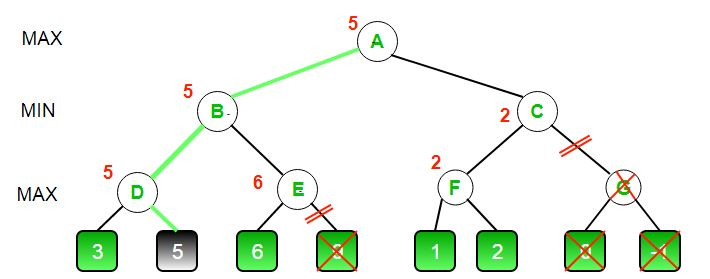
\includegraphics[width=0.9\textwidth]{./.img/alpha-beta.jpg}
                \caption{Ejemplo de poda Alpha-Beta}
            \end{figure}
          }
        \subsection*{Primera implementación}
          \begin{lstlisting}[language=Python, caption=Implementación inicial del agente Alpha-Beta]
          \end{lstlisting}
        \subsection*{Implementación final}
            \begin{lstlisting}[language=Python, caption=Implementación final del agente Alpha-Beta]
class AlphaBetaAgent(MultiAgentSearchAgent):
    """
    Implementacion del minimax con poda alfa-beta.
    """

    def getAction(self, gameState):
        """
        Devuelve la mejor acción para Pacman desde el estado actual `gameState` usando Minimax.
        """
        # Llama a la función minimax empezando con el agente 0 (Pacman) y profundidad 0
        best_action, _ = self.minimax(gameState, agentIndex=0, depth=0, alpha=float('-inf'), beta=float('inf'))
        return best_action

    def minimax(self, gameState, agentIndex, depth, alpha, beta):
        """
        Función minimax que devuelve la mejor acción y su valor para el agente actual.
        """
        # Si el estado es terminal (gana o pierde) o alcanzamos la profundidad máxima, evaluamos el estado
        if gameState.isWin() or gameState.isLose() or depth == self.depth:
            return None, self.evaluationFunction(gameState)

        if agentIndex == 0: # Pacman - Maximizador
            return self.max_value(gameState, agentIndex, depth, alpha, beta)
        else:               # Fantasmas - Minimizadores
            return self.min_value(gameState, agentIndex, depth, alpha, beta)

    def max_value(self, gameState, agentIndex, depth, alpha, beta):
        """
        Calcula el valor máximo para el agente Pacman (maximizador).
        """
        # Inicializar el mejor valor y la mejor acción
        best_value = float('-inf')
        best_action = None

        # Recorre todas las acciones legales para Pacman
        for action in gameState.getLegalActions(agentIndex):
            # Generar el estado sucesor
            successorState = gameState.generateSuccessor(agentIndex, action)
            # Calcular el valor del sucesor usando minimax con el siguiente agente
            _, successor_value = self.minimax(successorState, agentIndex + 1, depth, alpha, beta)
            # Actualiza el valor máximo si se encuentra un mejor valor
            if successor_value > best_value:
                best_value = successor_value
                best_action = action
                
            if best_value > beta:
                return best_action, best_value
            alpha = max(alpha, best_value)

        return best_action, best_value

    def min_value(self, gameState, agentIndex, depth, alpha, beta):
        """
        Calcula el valor mínimo para los fantasmas (minimizador).
        """
        # Inicializar el peor valor y la mejor acción
        worst_value = float('inf')
        best_action = None

        # Recorre todas las acciones legales para el fantasma actual
        for action in gameState.getLegalActions(agentIndex):
            # Generar el estado sucesor
            successorState = gameState.generateSuccessor(agentIndex, action)
            
            # Si es el último fantasma, pasamos a Pacman incrementando la profundidad
            if agentIndex == gameState.getNumAgents() - 1:
                # Calcula el valor del sucesor con Pacman y siguiente nivel de profundidad
                _, successor_value = self.minimax(successorState, 0, depth + 1, alpha, beta)
            else:
                # Calcula el valor del sucesor con el siguiente fantasma
                _, successor_value = self.minimax(successorState, agentIndex + 1, depth, alpha, beta)

            # Actualiza el valor mínimo si se encuentra un peor valor
            if successor_value < worst_value:
                worst_value = successor_value
                best_action = action
                
            if worst_value < alpha:
                return best_action, worst_value
            beta = min(beta, worst_value)

        return best_action, worst_value
            \end{lstlisting}
        \subsection*{Comentarios}
          \paragraph*{}{

          }
      \clearpage\section{Expectimax}
        \subsection*{Descripción}
          \paragraph*{}{
            El algoritmo Expectimax es una variante del algoritmo Minimax que se utiliza cuando los oponentes no toman siempre la mejor decisión posible.
            En lugar de minimizar el valor de los nodos de los oponentes, el algoritmo Expectimax toma la media de los valores de los nodos sucesores.
          }
        \subsection*{Primera implementación}
          \begin{lstlisting}[language=Python, caption=Implementación inicial del agente Expectimax]
class ExpectimaxAgent(MultiAgentSearchAgent):
    """
      Implementacion del algoritmo Expectimax.
    """

    def getAction(self, gameState):
        return self.expectimax(gameState, agentIndex=0, depth=0)
    
    def expectimax(self, gameState, agentIndex, depth):
        """
        Función expectimax que devuelve la mejor acción y su valor para el agente actual.
        """
        # Si el estado es terminal (gana o pierde) o alcanzamos la profundidad máxima, evaluamos el estado
        if gameState.isWin() or gameState.isLose() or depth == self.depth:
            return None, self.evaluationFunction(gameState)

        if agentIndex == 0: # Pacman - Maximizador
            return self.max_value(gameState, agentIndex, depth)
        else:               # Fantasmas - Minimizadores
            return self.exp_value(gameState, agentIndex, depth)
        
    def max_value(self, gameState, agentIndex, depth):
        """
        Calcula el valor máximo para el agente Pacman (maximizador).
        """
        # Inicializar el mejor valor y la mejor acción
        best_value = float('-inf')
        best_action = None

        # Recorre todas las acciones legales para Pacman
        for action in gameState.getLegalActions(agentIndex):
            # Generar el estado sucesor
            successorState = gameState.generateSuccessor(agentIndex, action)
            # Calcular el valor del sucesor usando expectimax con el siguiente agente
            _, successor_value = self.expectimax(successorState, agentIndex + 1, depth)
            # Actualiza el valor máximo si se encuentra un mejor valor
            if successor_value > best_value:
                best_value = successor_value
                best_action = action

        return best_action, best_value
    
    def exp_value(self, gameState, agentIndex, depth):
        """
        Calcula el valor esperado para los fantasmas (minimizador).
        """
        # Inicializar el valor esperado y la mejor acción
        expected_value = 0
        best_action = None

        # Recorre todas las acciones legales para el fantasma actual
        for action in gameState.getLegalActions(agentIndex):
            # Generar el estado sucesor
            successorState = gameState.generateSuccessor(agentIndex, action)
            
            # Si es el último fantasma, pasamos a Pacman incrementando la profundidad
            if agentIndex == gameState.getNumAgents() - 1:
                # Calcula el valor del sucesor con Pacman y siguiente nivel de profundidad
                _, successor_value = self.expectimax(successorState, 0, depth + 1)
            else:
                # Calcula el valor del sucesor con el siguiente fantasma
                _, successor_value = self.expectimax(successorState, agentIndex + 1, depth)
            
            # Actualiza el valor esperado con el valor del sucesor
            expected_value += successor_value / len(gameState.getLegalActions(agentIndex))

        return best_action, expected_value
          \end{lstlisting}
        \subsection*{Implementación final}
            \begin{lstlisting}[language=Python, caption=Implementación final del agente Expectimax]
class ExpectimaxAgent(MultiAgentSearchAgent):
    """
        Implementacion del algoritmo Expectimax.
    """

    def getAction(self, gameState):
        best_action, _ = self.expectimax(gameState, agentIndex=0, depth=0)
        return best_action
    
    def expectimax(self, gameState, agentIndex, depth):
        """
        Función expectimax que devuelve la mejor acción y su valor para el agente actual.
        """
        # Si el estado es terminal (gana o pierde) o alcanzamos la profundidad máxima, evaluamos el estado
        if gameState.isWin() or gameState.isLose() or depth == self.depth:
            return None, self.evaluationFunction(gameState)

        if agentIndex == 0: # Pacman - Maximizador
            return self.max_value(gameState, agentIndex, depth)
        else:               # Fantasmas - Minimizadores
            return self.exp_value(gameState, agentIndex, depth)
        
    def max_value(self, gameState, agentIndex, depth):
        """
        Calcula el valor máximo para el agente Pacman (maximizador).
        """
        # Inicializar el mejor valor y la mejor acción
        best_value = float('-inf')
        best_action = None

        # Recorre todas las acciones legales para Pacman
        for action in gameState.getLegalActions(agentIndex):
            # Generar el estado sucesor
            successorState = gameState.generateSuccessor(agentIndex, action)
            # Calcular el valor del sucesor usando expectimax con el siguiente agente
            _, successor_value = self.expectimax(successorState, agentIndex + 1, depth)
            # Actualiza el valor máximo si se encuentra un mejor valor
            if successor_value > best_value:
                best_value = successor_value
                best_action = action

        return best_action, best_value
    
    def exp_value(self, gameState, agentIndex, depth):
        """
        Calcula el valor esperado para los fantasmas (minimizador).
        """
        # Inicializar el valor esperado y la mejor acción
        expected_value = 0
        best_action = None

        # Recorre todas las acciones legales para el fantasma actual
        actions = gameState.getLegalActions(agentIndex)
        for action in actions:
            # Generar el estado sucesor
            successorState = gameState.generateSuccessor(agentIndex, action)
            
            # Si es el último fantasma, pasamos a Pacman incrementando la profundidad
            if agentIndex == gameState.getNumAgents() - 1:
                # Calcula el valor del sucesor con Pacman y siguiente nivel de profundidad
                _, successor_value = self.expectimax(successorState, 0, depth + 1)
            else:
                # Calcula el valor del sucesor con el siguiente fantasma
                _, successor_value = self.expectimax(successorState, agentIndex + 1, depth)
            # Actualiza el valor esperado con el valor del sucesor
            expected_value += successor_value / len(actions)

        return best_action, expected_value            
            \end{lstlisting}
        \subsection*{Comentarios}
          \paragraph*{}{

          }
      \clearpage\section{Función de Evaluación}
        \subsection*{Descripción}
          \paragraph*{}{
            Este ejercicio, consiste en mejorar la función de evaluación del agente reflex. 
            La función de evaluación asigna un valor numérico a cada estado, y el agente selecciona la acción que maximiza este valor. 
            Para mejorar la implementación previa unicamente se han añadido más factores a tener en cuenta en la evaluación de los estados.
            Para asignar un valor a cada estado, la función de evaluación considera varios factores, como la distancia a la comida, la proximidad a los fantasmas y la cantidad de comida restante.
          }
        \subsection*{Primera implementación}
          \begin{lstlisting}[language=Python, caption=Implementación inicial de la función de evaluación]
          \end{lstlisting}
        \subsection*{Implementación final}
          \begin{lstlisting}[language=Python, caption=Implementación final de la función de evaluación]
def betterEvaluationFunction(currentGameState):
    """
    Función de evaluación para Pacman que considera múltiples factores del estado de juego.
    """

    # Obtener el estado actual de Pacman
    pacmanPos = currentGameState.getPacmanPosition()
    
    # Obtener la comida restante y convertirla a una lista de posiciones
    food = currentGameState.getFood().asList()
    
    # Obtener las posiciones de los fantasmas y sus estados (asustados o no)
    ghostStates = currentGameState.getGhostStates()
    ghostPositions = [ghost.getPosition() for ghost in ghostStates]
    scaredTimes = [ghostState.scaredTimer for ghostState in ghostStates]
    
    # Obtener las pelets de poder restantes
    capsules = currentGameState.getCapsules()
    
    # Obtener el puntaje actual del juego
    score = currentGameState.getScore()
    
    # Inicializar la evaluación con el puntaje actual
    evaluation = score

    # 1. Distancia a la comida: Minimizar la distancia a la comida
    if food:
        minFoodDist = min([manhattanDistance(pacmanPos, foodPos) for foodPos in food])
        # Dar un peso inversamente proporcional a la distancia a la comida
        evaluation += 1.0 / (minFoodDist + 1)  # Sumar al score, +1 para evitar división por 0

    # 2. Distancia a los fantasmas: Maximizar la distancia a los fantasmas (si no están asustados)
    for i, ghostPos in enumerate(ghostPositions):
        ghostDist = manhattanDistance(pacmanPos, ghostPos)
        
        if scaredTimes[i] > 0:  # Fantasma asustado
            # Acercarse a los fantasmas asustados para ganar puntos al comérselos
            evaluation += 10.0 / (ghostDist + 1)  # Dar un peso a la proximidad a fantasmas asustados
        else:  # Fantasma no asustado
            # Alejarse de los fantasmas si están demasiado cerca
            if ghostDist > 0:
                evaluation -= 10.0 / ghostDist  # Penalizar por estar cerca de un fantasma peligroso

    # 3. Comida restante: Cuanta menos comida quede, mejor es el estado
    evaluation -= 4.0 * len(food)  # Penalizar más comida restante

    # 4. Cápsulas de poder: Incentivar estar cerca de las pelets de poder
    if capsules:
        minCapsuleDist = min([manhattanDistance(pacmanPos, capsule) for capsule in capsules])
        evaluation += 5.0 / (minCapsuleDist + 1)  # Dar un peso inverso a la distancia a las pelets
        evaluation -= 100 * len(capsules)  # Penalizar si quedan muchas pelets sin recoger

    # Devolver la evaluación final ajustada por todos los factores
    return evaluation
        
          \end{lstlisting}
        \subsection*{Comentarios}
    \chapter{Resultados}
      \section{Casos de prueba}
      \clearpage\section{Autograder}
        \begin{lstlisting}[language=Python, caption=Resultados del Autograder]
Starting on 10-15 at 18:32:26

Question q1
===========

Pacman emerges victorious! Score: 1238
Pacman emerges victorious! Score: 1244
Pacman emerges victorious! Score: 1239
Pacman emerges victorious! Score: 1235
Pacman emerges victorious! Score: 1233
Pacman emerges victorious! Score: 1241
Pacman emerges victorious! Score: 1246
Pacman emerges victorious! Score: 1242
Pacman emerges victorious! Score: 1239
Pacman emerges victorious! Score: 1242
Average Score: 1239.9
Scores:        1238.0, 1244.0, 1239.0, 1235.0, 1233.0, 1241.0, 1246.0, 1242.0, 1239.0, 1242.0
Win Rate:      10/10 (1.00)
Record:        Win, Win, Win, Win, Win, Win, Win, Win, Win, Win
*** PASS: test_cases/q1/grade-agent.test (4 of 4 points)
***     1239.9 average score (2 of 2 points)
***         Grading scheme:
***          < 500:  0 points
***         >= 500:  1 points
***         >= 1000:  2 points
***     10 games not timed out (0 of 0 points)
***         Grading scheme:
***          < 10:  fail
***         >= 10:  0 points
***     10 wins (2 of 2 points)
***         Grading scheme:
***          < 1:  fail
***         >= 1:  0 points
***         >= 5:  1 points
***         >= 10:  2 points

### Question q1: 4/4 ###


Question q2
===========

*** PASS: test_cases/q2/0-eval-function-lose-states-1.test
*** PASS: test_cases/q2/0-eval-function-lose-states-2.test
*** PASS: test_cases/q2/0-eval-function-win-states-1.test
*** PASS: test_cases/q2/0-eval-function-win-states-2.test
*** PASS: test_cases/q2/0-lecture-6-tree.test
*** PASS: test_cases/q2/0-small-tree.test
*** PASS: test_cases/q2/1-1-minmax.test
*** PASS: test_cases/q2/1-2-minmax.test
*** PASS: test_cases/q2/1-3-minmax.test
*** PASS: test_cases/q2/1-4-minmax.test
*** PASS: test_cases/q2/1-5-minmax.test
*** PASS: test_cases/q2/1-6-minmax.test
*** PASS: test_cases/q2/1-7-minmax.test
*** PASS: test_cases/q2/1-8-minmax.test
*** PASS: test_cases/q2/2-1a-vary-depth.test
*** PASS: test_cases/q2/2-1b-vary-depth.test
*** PASS: test_cases/q2/2-2a-vary-depth.test
*** PASS: test_cases/q2/2-2b-vary-depth.test
*** PASS: test_cases/q2/2-3a-vary-depth.test
*** PASS: test_cases/q2/2-3b-vary-depth.test
*** PASS: test_cases/q2/2-4a-vary-depth.test
*** PASS: test_cases/q2/2-4b-vary-depth.test
*** PASS: test_cases/q2/2-one-ghost-3level.test
*** PASS: test_cases/q2/3-one-ghost-4level.test
*** PASS: test_cases/q2/4-two-ghosts-3level.test
*** PASS: test_cases/q2/5-two-ghosts-4level.test
*** PASS: test_cases/q2/6-tied-root.test
*** PASS: test_cases/q2/7-1a-check-depth-one-ghost.test
*** PASS: test_cases/q2/7-1b-check-depth-one-ghost.test
*** PASS: test_cases/q2/7-1c-check-depth-one-ghost.test
*** PASS: test_cases/q2/7-2a-check-depth-two-ghosts.test
*** PASS: test_cases/q2/7-2b-check-depth-two-ghosts.test
*** PASS: test_cases/q2/7-2c-check-depth-two-ghosts.test
*** Running MinimaxAgent on smallClassic 1 time(s).
Pacman died! Score: 84
Average Score: 84.0
Scores:        84.0
Win Rate:      0/1 (0.00)
Record:        Loss
*** Finished running MinimaxAgent on smallClassic after 0.7832581996917725 seconds.
*** Won 0 out of 1 games. Average score: 84.0 ***
*** PASS: test_cases/q2/8-pacman-game.test

### Question q2: 5/5 ###


Question q3
===========

*** PASS: test_cases/q3/0-eval-function-lose-states-1.test
*** PASS: test_cases/q3/0-eval-function-lose-states-2.test
*** PASS: test_cases/q3/0-eval-function-win-states-1.test
*** PASS: test_cases/q3/0-eval-function-win-states-2.test
*** PASS: test_cases/q3/0-lecture-6-tree.test
*** PASS: test_cases/q3/0-small-tree.test
*** PASS: test_cases/q3/1-1-minmax.test
*** PASS: test_cases/q3/1-2-minmax.test
*** PASS: test_cases/q3/1-3-minmax.test
*** PASS: test_cases/q3/1-4-minmax.test
*** PASS: test_cases/q3/1-5-minmax.test
*** PASS: test_cases/q3/1-6-minmax.test
*** PASS: test_cases/q3/1-7-minmax.test
*** PASS: test_cases/q3/1-8-minmax.test
*** PASS: test_cases/q3/2-1a-vary-depth.test
*** PASS: test_cases/q3/2-1b-vary-depth.test
*** PASS: test_cases/q3/2-2a-vary-depth.test
*** PASS: test_cases/q3/2-2b-vary-depth.test
*** PASS: test_cases/q3/2-3a-vary-depth.test
*** PASS: test_cases/q3/2-3b-vary-depth.test
*** PASS: test_cases/q3/2-4a-vary-depth.test
*** PASS: test_cases/q3/2-4b-vary-depth.test
*** PASS: test_cases/q3/2-one-ghost-3level.test
*** PASS: test_cases/q3/3-one-ghost-4level.test
*** PASS: test_cases/q3/4-two-ghosts-3level.test
*** PASS: test_cases/q3/5-two-ghosts-4level.test
*** PASS: test_cases/q3/6-tied-root.test
*** PASS: test_cases/q3/7-1a-check-depth-one-ghost.test
*** PASS: test_cases/q3/7-1b-check-depth-one-ghost.test
*** PASS: test_cases/q3/7-1c-check-depth-one-ghost.test
*** PASS: test_cases/q3/7-2a-check-depth-two-ghosts.test
*** PASS: test_cases/q3/7-2b-check-depth-two-ghosts.test
*** PASS: test_cases/q3/7-2c-check-depth-two-ghosts.test
*** Running AlphaBetaAgent on smallClassic 1 time(s).
Pacman died! Score: 84
Average Score: 84.0
Scores:        84.0
Win Rate:      0/1 (0.00)
Record:        Loss
*** Finished running AlphaBetaAgent on smallClassic after 0.7023296356201172 seconds.
*** Won 0 out of 1 games. Average score: 84.0 ***
*** PASS: test_cases/q3/8-pacman-game.test

### Question q3: 5/5 ###


Question q4
===========

*** PASS: test_cases/q4/0-eval-function-lose-states-1.test
*** PASS: test_cases/q4/0-eval-function-lose-states-2.test
*** PASS: test_cases/q4/0-eval-function-win-states-1.test
*** PASS: test_cases/q4/0-eval-function-win-states-2.test
*** PASS: test_cases/q4/0-expectimax1.test
*** PASS: test_cases/q4/1-expectimax2.test
*** PASS: test_cases/q4/2-one-ghost-3level.test
*** PASS: test_cases/q4/3-one-ghost-4level.test
*** PASS: test_cases/q4/4-two-ghosts-3level.test
*** PASS: test_cases/q4/5-two-ghosts-4level.test
*** PASS: test_cases/q4/6-1a-check-depth-one-ghost.test
*** PASS: test_cases/q4/6-1b-check-depth-one-ghost.test
*** PASS: test_cases/q4/6-1c-check-depth-one-ghost.test
*** PASS: test_cases/q4/6-2a-check-depth-two-ghosts.test
*** PASS: test_cases/q4/6-2b-check-depth-two-ghosts.test
*** PASS: test_cases/q4/6-2c-check-depth-two-ghosts.test
*** Running ExpectimaxAgent on smallClassic 1 time(s).
Pacman died! Score: 84
Average Score: 84.0
Scores:        84.0
Win Rate:      0/1 (0.00)
Record:        Loss
*** Finished running ExpectimaxAgent on smallClassic after 0.8156166076660156 seconds.
*** Won 0 out of 1 games. Average score: 84.0 ***
*** PASS: test_cases/q4/7-pacman-game.test

### Question q4: 5/5 ###


Question q5
===========

Pacman emerges victorious! Score: 1366
Pacman emerges victorious! Score: 1026
Pacman emerges victorious! Score: 1060
Pacman emerges victorious! Score: 1089
Pacman emerges victorious! Score: 1015
Pacman emerges victorious! Score: 1016
Pacman emerges victorious! Score: 1238
Pacman emerges victorious! Score: 760
Pacman emerges victorious! Score: 1372
Pacman emerges victorious! Score: 1321
Average Score: 1126.3
Scores:        1366.0, 1026.0, 1060.0, 1089.0, 1015.0, 1016.0, 1238.0, 760.0, 1372.0, 1321.0
Win Rate:      10/10 (1.00)
Record:        Win, Win, Win, Win, Win, Win, Win, Win, Win, Win
*** PASS: test_cases/q5/grade-agent.test (6 of 6 points)
***     1126.3 average score (2 of 2 points)
***         Grading scheme:
***          < 500:  0 points
***         >= 500:  1 points
***         >= 1000:  2 points
***     10 games not timed out (1 of 1 points)
***         Grading scheme:
***          < 0:  fail
***         >= 0:  0 points
***         >= 10:  1 points
***     10 wins (3 of 3 points)
***         Grading scheme:
***          < 1:  fail
***         >= 1:  1 points
***         >= 5:  2 points
***         >= 10:  3 points

### Question q5: 6/6 ###


Finished at 18:32:43

Provisional grades
==================
Question q1: 4/4
Question q2: 5/5
Question q3: 5/5
Question q4: 5/5
Question q5: 6/6
------------------
Total: 25/25

Your grades are NOT yet registered.  To register your grades, make sure
to follow your instructor's guidelines to receive credit on your project.


        \end{lstlisting}
\end{document}